\section*{Resolução da Questão 1: Algoritmos de Busca em Grafos}

\subsection*{A) Estruturação do Problema}

A definição deste desafio de busca em espaço de estados baseia-se nos seguintes elementos essenciais:

\begin{itemize}
    \item \textbf{Representação do Estado Atual}: Uma letra ou string que identifica o aposento atual do agente. Por exemplo: $s \in \{A, B, C, \dots, S\}$.
    \item \textbf{Estado de Origem}: O ponto de partida do labirinto é a sala $A$, portanto $s_0 = A$.
    \item \textbf{Verificação de Conclusão}: Condição que testa se a sala atual $s$ corresponde ao alvo $S$. A função $ChegouAoFim(s)$ retorna $Verdadeiro$ caso $s = S$, e $Falso$ em outras situações.
    \item \textbf{Transições Possíveis (Sucessores)}: Função que mapeia os deslocamentos válidos a partir de uma sala $s$ para as adjacentes, seguindo rigidamente a ordem alfabética. Ex: $Vizinhos(A) = \{B, C, D\}$, $Vizinhos(B) = \{E, F\}$.
    \item \textbf{Métrica de Custo}: O custo associado à transição entre duas salas conectadas. Sendo um movimento de custo uniforme, $c(s, a, s') = 1$. O custo total é a quantidade de passos dados.
\end{itemize}

\textbf{Definição do Grafo em Python:}
\begin{lstlisting}[language=Python]
adjacency_map = {
    'A': ['B', 'C', 'D'], 'B': ['E', 'F'], 'C': ['G', 'H'],
    'D': ['I'], 'E': ['J'], 'F': ['K', 'L'], 'G': ['M'],
    'H': ['N', 'O'], 'I': ['P'], 'J': [], 'K': ['Q'],
    'L': [], 'M': ['R'], 'N': [], 'O': ['S'], 'P': [],
    'Q': [], 'R': [], 'S': []
}
start_node = 'A'
target_node = 'S'
\end{lstlisting}

\subsection*{B) Avaliação dos Métodos de Busca}

\subsubsection*{1. Busca em Largura (BFS)}

\textbf{Desempenho da BFS:}
\begin{itemize}
    \item \textbf{Trajeto da Solução:} A $\rightarrow$ C $\rightarrow$ H $\rightarrow$ O $\rightarrow$ S
    \item \textbf{Custo Total:} 4
    \item \textbf{Nível de Profundidade:} 4
    \item \textbf{Quantidade de Nós Expandidos:} 15
    \item \textbf{Quantidade de Nós Gerados:} 19
\end{itemize}

\textbf{Acompanhamento da Execução (Fronteira FIFO):}
\begin{table}[h!]
\centering
\begin{tabular}{|c|c|l|}
\hline
\textbf{Iteração} & \textbf{Nó Processado} & \textbf{Estado da Fronteira Pós-Expansão} \\ \hline
1 & A & [B, C, D] \\ \hline
2 & B & [C, D, E, F] \\ \hline
3 & C & [D, E, F, G, H] \\ \hline
4 & D & [E, F, G, H, I] \\ \hline
5 & E & [F, G, H, I, J] \\ \hline
6 & F & [G, H, I, J, K, L] \\ \hline
7 & G & [H, I, J, K, L, M] \\ \hline
8 & H & [I, J, K, L, M, N, O] \\ \hline
9 & I & [J, K, L, M, N, O, P] \\ \hline
10 & J & [K, L, M, N, O, P] \\ \hline
11 & K & [L, M, N, O, P, Q] \\ \hline
12 & L & [M, N, O, P, Q] \\ \hline
13 & M & [N, O, P, Q, R] \\ \hline
14 & N & [O, P, Q, R] \\ \hline
15 & O & [P, Q, R, S] \\ \hline
16 & S & Sucesso (Objetivo Encontrado) \\ \hline
\end{tabular}
\end{table}

\textbf{Árvore de Exploração Parcial (BFS):}
\textit{Nota: Nós preenchidos em ciano (\textcolor{cyan}{Cor}) indicam expansão. O alvo é laranja (\textcolor{orange}{Cor}). Círculos vazios apenas gerados.}

\begin{center}
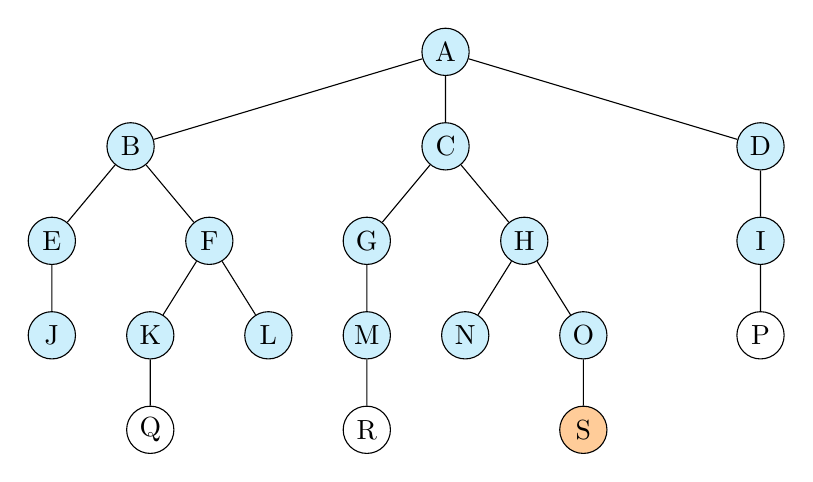
\begin{tikzpicture}[level distance=1.2cm,
  level 1/.style={sibling distance=4cm},
  level 2/.style={sibling distance=2cm},
  level 3/.style={sibling distance=1.5cm},
  every node/.style={circle, draw, minimum size=0.6cm, inner sep=1pt}]
  
  \node[fill=cyan!20] {A}
    child {node[fill=cyan!20] {B}
      child {node[fill=cyan!20] {E}
        child {node[fill=cyan!20] {J}}
      }
      child {node[fill=cyan!20] {F}
        child {node[fill=cyan!20] {K}
          child {node {Q}}
        }
        child {node[fill=cyan!20] {L}}
      }
    }
    child {node[fill=cyan!20] {C}
      child {node[fill=cyan!20] {G}
        child {node[fill=cyan!20] {M}
          child {node {R}}
        }
      }
      child {node[fill=cyan!20] {H}
        child {node[fill=cyan!20] {N}}
        child {node[fill=cyan!20] {O}
          child {node[fill=orange!40] {S}}
        }
      }
    }
    child {node[fill=cyan!20] {D}
      child {node[fill=cyan!20] {I}
        child {node {P}}
      }
    };
\end{tikzpicture}
\end{center}

\subsubsection*{2. Busca em Profundidade (DFS)}

Para garantir que a DFS priorize os vizinhos iniciais (por exemplo, visitar B antes de C ou D), a fronteira do tipo Pilha insere os elementos em ordem reversa: D, depois C, depois B.

\textbf{Desempenho da DFS:}
\begin{itemize}
    \item \textbf{Trajeto da Solução:} A $\rightarrow$ C $\rightarrow$ H $\rightarrow$ O $\rightarrow$ S
    \item \textbf{Custo Total:} 4
    \item \textbf{Nível de Profundidade:} 4
    \item \textbf{Quantidade de Nós Expandidos:} 15
    \item \textbf{Quantidade de Nós Gerados:} 17
\end{itemize}

\textbf{Acompanhamento da Execução (Fronteira LIFO):}
\begin{table}[h!]
\centering
\begin{tabular}{|c|c|l|}
\hline
\textbf{Iteração} & \textbf{Nó Processado} & \textbf{Estado da Fronteira Pós-Expansão} \\ \hline
1 & A & [D, C, B] \\ \hline
2 & B & [D, C, F, E] \\ \hline
3 & E & [D, C, F, J] \\ \hline
4 & J & [D, C, F] \\ \hline
5 & F & [D, C, L, K] \\ \hline
6 & K & [D, C, L, Q] \\ \hline
7 & Q & [D, C, L] \\ \hline
8 & L & [D, C] \\ \hline
9 & C & [D, H, G] \\ \hline
10 & G & [D, H, M] \\ \hline
11 & M & [D, H, R] \\ \hline
12 & R & [D, H] \\ \hline
13 & H & [D, O, N] \\ \hline
14 & N & [D, O] \\ \hline
15 & O & [D, S] \\ \hline
16 & S & Sucesso (Objetivo Encontrado) \\ \hline
\end{tabular}
\end{table}

\textbf{Árvore de Exploração Parcial (DFS):}

\begin{center}
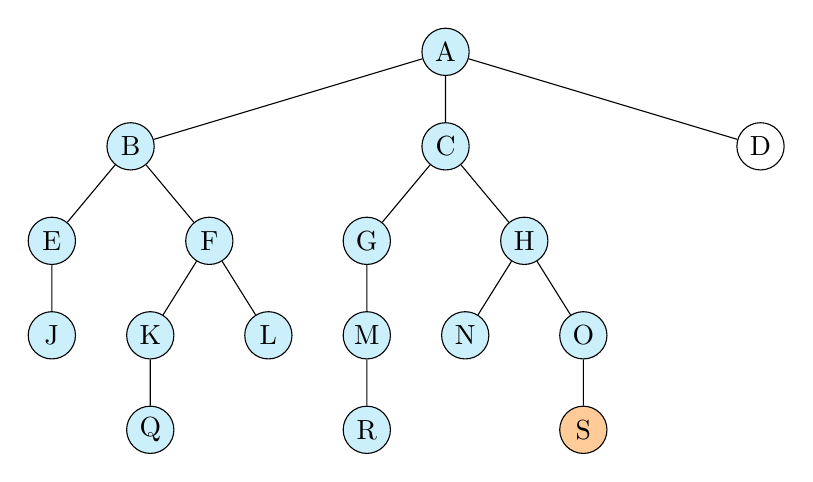
\begin{tikzpicture}[level distance=1.2cm,
  level 1/.style={sibling distance=4cm},
  level 2/.style={sibling distance=2cm},
  level 3/.style={sibling distance=1.5cm},
  every node/.style={circle, draw, minimum size=0.6cm, inner sep=1pt}]
  
  \node[fill=cyan!20] {A}
    child {node[fill=cyan!20] {B}
      child {node[fill=cyan!20] {E}
        child {node[fill=cyan!20] {J}}
      }
      child {node[fill=cyan!20] {F}
        child {node[fill=cyan!20] {K}
          child {node[fill=cyan!20] {Q}}
        }
        child {node[fill=cyan!20] {L}}
      }
    }
    child {node[fill=cyan!20] {C}
      child {node[fill=cyan!20] {G}
        child {node[fill=cyan!20] {M}
          child {node[fill=cyan!20] {R}}
        }
      }
      child {node[fill=cyan!20] {H}
        child {node[fill=cyan!20] {N}}
        child {node[fill=cyan!20] {O}
          child {node[fill=orange!40] {S}}
        }
      }
    }
    child {node {D}};
\end{tikzpicture}
\end{center}

\subsubsection*{3. Busca de Aprofundamento Iterativo (IDS)}

A estratégia IDS repete sondagens em profundidade limitada (DLS) nos limiares de $L=0$ até $L=4$, onde o objetivo $S$ é enfim descoberto.

\textbf{Desempenho da IDS:}
\begin{itemize}
    \item \textbf{Trajeto da Solução:} A $\rightarrow$ C $\rightarrow$ H $\rightarrow$ O $\rightarrow$ S
    \item \textbf{Custo Total:} 4
    \item \textbf{Nós Expandidos (Soma Global):} 27
    \item \textbf{Nós Gerados (Soma Global):} 47
\end{itemize}

O progresso repete a lógica até o limite 4. A árvore gerada no último limite ($L=4$) é idêntica à porção da árvore de DFS que alcança profundidade 4, resultando na mesma tabela observada para DFS.

\subsection*{C) Algoritmos em Linguagem Python}

O código-fonte com as implementações encontra-se na seção de Anexos do trabalho.

\subsection*{D) Experimento: Ordem de Geração Invertida C $\rightarrow$ H, G}

Ao modificar estritamente a prioridade dos vizinhos de C de \texttt{(G, H)} para \texttt{(H, G)}, o comportamento de percurso se ajusta. 

\subsubsection*{1. Nova Execução de BFS}
\begin{table}[h!]
\centering
\begin{tabular}{|c|c|l|}
\hline
\textbf{Iteração} & \textbf{Nó Processado} & \textbf{Estado da Fronteira Pós-Expansão} \\ \hline
1 & A & [B, C, D] \\ \hline
2 & B & [C, D, E, F] \\ \hline
3 & C & [D, E, F, H, G] \\ \hline
4 & D & [E, F, H, G, I] \\ \hline
5 & E & [F, H, G, I, J] \\ \hline
6 & F & [H, G, I, J, K, L] \\ \hline
7 & H & [G, I, J, K, L, N, O] \\ \hline
8 & G & [I, J, K, L, N, O, M] \\ \hline
9 & I & [J, K, L, N, O, M, P] \\ \hline
10 & J & [K, L, N, O, M, P] \\ \hline
11 & K & [L, N, O, M, P] \\ \hline
12 & L & [N, O, M, P, Q] \\ \hline
13 & N & [O, M, P, Q] \\ \hline
14 & O & [M, P, Q, S] \\ \hline
15 & S & Sucesso (Objetivo Encontrado) \\ \hline
\end{tabular}
\end{table}

\begin{center}
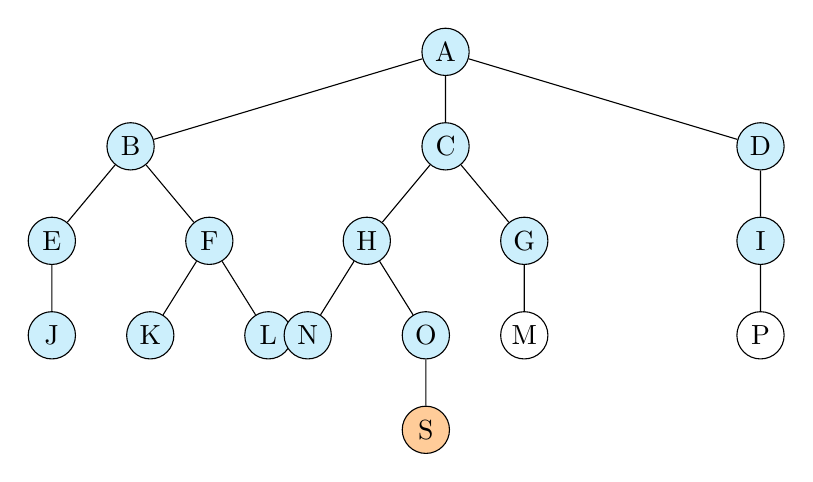
\begin{tikzpicture}[level distance=1.2cm, level 1/.style={sibling distance=4cm}, level 2/.style={sibling distance=2cm}, level 3/.style={sibling distance=1.5cm},
  every node/.style={circle, draw, minimum size=0.6cm, inner sep=1pt}]
  \node[fill=cyan!20] {A}
    child {node[fill=cyan!20] {B}
      child {node[fill=cyan!20] {E} child {node[fill=cyan!20] {J}}}
      child {node[fill=cyan!20] {F} child {node[fill=cyan!20] {K}} child {node[fill=cyan!20] {L}}}
    }
    child {node[fill=cyan!20] {C}
      child {node[fill=cyan!20] {H} child {node[fill=cyan!20] {N}} child {node[fill=cyan!20] {O} child {node[fill=orange!40] {S}}}}
      child {node[fill=cyan!20] {G} child {node {M}}}
    }
    child {node[fill=cyan!20] {D}
      child {node[fill=cyan!20] {I} child {node {P}}}
    };
\end{tikzpicture}
\end{center}

\subsubsection*{2. Nova Execução de DFS}
\begin{table}[h!]
\centering
\begin{tabular}{|c|c|l|}
\hline
\textbf{Iteração} & \textbf{Nó Processado} & \textbf{Estado da Fronteira Pós-Expansão} \\ \hline
1 & A & [D, C, B] \\ \hline
2 & B & [D, C, F, E] \\ \hline
3 & E & [D, C, F, J] \\ \hline
4 & J & [D, C, F] \\ \hline
5 & F & [D, C, L, K] \\ \hline
6 & K & [D, C, L, Q] \\ \hline
7 & Q & [D, C, L] \\ \hline
8 & L & [D, C] \\ \hline
9 & C & [D, G, H] \\ \hline
10 & H & [D, G, O, N] \\ \hline
11 & N & [D, G, O] \\ \hline
12 & O & [D, G, S] \\ \hline
13 & S & Sucesso (Objetivo Encontrado) \\ \hline
\end{tabular}
\end{table}

\begin{center}
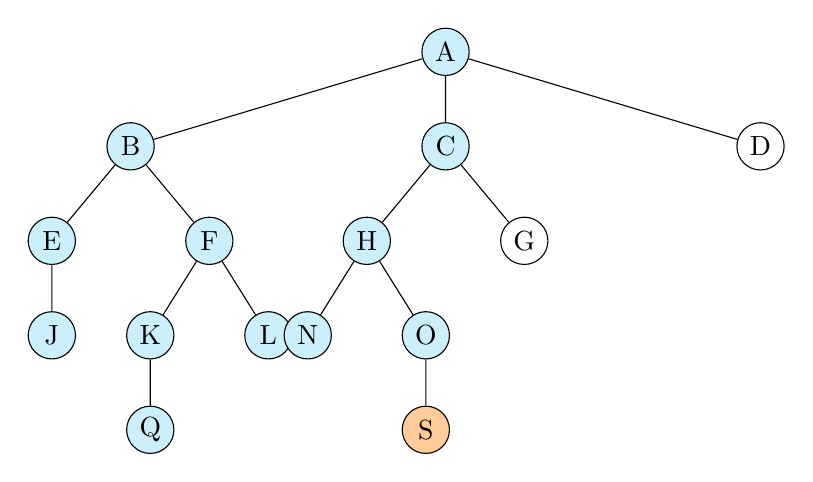
\begin{tikzpicture}[level distance=1.2cm, level 1/.style={sibling distance=4cm}, level 2/.style={sibling distance=2cm}, level 3/.style={sibling distance=1.5cm},
  every node/.style={circle, draw, minimum size=0.6cm, inner sep=1pt}]
  \node[fill=cyan!20] {A}
    child {node[fill=cyan!20] {B}
      child {node[fill=cyan!20] {E} child {node[fill=cyan!20] {J}}}
      child {node[fill=cyan!20] {F} child {node[fill=cyan!20] {K} child {node[fill=cyan!20] {Q}}} child {node[fill=cyan!20] {L}}}
    }
    child {node[fill=cyan!20] {C}
      child {node[fill=cyan!20] {H} child {node[fill=cyan!20] {N}} child {node[fill=cyan!20] {O} child {node[fill=orange!40] {S}}}}
      child {node {G}}
    }
    child {node {D}};
\end{tikzpicture}
\end{center}

\subsubsection*{Conclusões do Experimento}
\begin{enumerate}[label=\roman*)]
    \item O percurso ótimo ($A \rightarrow C \rightarrow H \rightarrow O \rightarrow S$) foi mantido idêntico em todas as variantes.
    \item Ocorreu uma otimização nos nós expandidos em todas as técnicas.
    \item A Busca em Profundidade sofreu impacto tremendo (reduzindo a exploração inútil do ramo G de forma precoce).
    \item A Amplitude manteve-se como a técnica mais punitiva em RAM devido à retenção dos irmãos não-visitados de nível.
\end{enumerate}

\subsection*{E) Avaliação e Comparativo}

A DFS demonstrou forte dependência de ordenação arbitrária para sua eficiência de curto prazo, enquanto a BFS é mecanicamente imune a ordenações em termos de garantia de profundidade mínima, mas extremamente custosa em cenários reais com amplo fator de ramificação. A IDS desponta como a escolha teórica mais robusta na preservação de RAM com exploração sistêmica controlada.
